In a first application of our extrapolation framework, we want to extrapolate the ground state energies of the nuclei \n{2}{H}, \n{3}{H} and \n{4}{He}, which were already used in the network training and analyze the extrapolation values in dependency on the maximum $N_\mathrm{max}$ of the input sequences. Instead of the many used interactions in the training, we decide on one interaction which will be used as a benchmark to compare this basic extrapolation framework to our more sophisticated methods which will be introduced in the later chapters. We decide on a semi-local momentum space regulated interaction of chiral order 2 with two body interactions and a cutoff at \SI{450}{\mega\electronvolt}. Since this interaction is different to the interactions used in training, we hope to see if the networks captured the characteristics which are own to the nuclei and reproduce those by extrapolating the results of previously unseen interactions.

To investigate the effects of an SRG evolution of the hamiltonian on the extrapolation results, we will further consider the above interaction in the case of an SRG evolution with a paramer of \srg{0.04} and \srg{0.08}.

\section{Results}
In \autoref{fig:eval_vanilla}, the evaluation of the interaction introduced above is shown for the three training nuclei.

% Varbound
An important metric in assessing our extrapolation comes from the variational principles of NCSM calculations for ground-state energies. Since the energies decrease mononously with increasing model-space dimensions, it is guarantied that the exact ground-state energy is lower than all computed NCSM values, regardless of model-space dimension. As a consequence, we can require from a reasonable extrapolation, that the extrapolated energy is lower than the lowest value at the maximum $N_\mathrm{max}$. This mimimum value is called the \textit{variational boundary}. For all maximum $N_\mathrm{max}$ in \autoref{fig:eval_vanilla}, those variational boundaries are shown as dashed lines. We can see that this condition is fulfilled for all nuclei in the case of a flow parameter of \srg{0.04}. This condition only fails for the extrapolations of \n{2}{H} with a flow parameter of \srg{0.08}. Additionally, we can also compare the extrapolation result to the variational boundary of the highest $N_\mathrm{max}$ available, as this provides a further upper bound for the exact ground-state energy. This upper bound is also interesting because it is not directly nor indirectly input into the networks, in contrast to the variational boundaries at the maximum $N_\mathrm{max}$, and thus represents a stronger condition for the extrapolation quality of the networks. For the nuclei \n{3}{H} and \n{4}{He}, this condition is also fulfilled. The extrapolations of the energies for the \n{2}{H} nucleus consistently fail to meet this condition.

\begin{figure}[H]
  \centering
  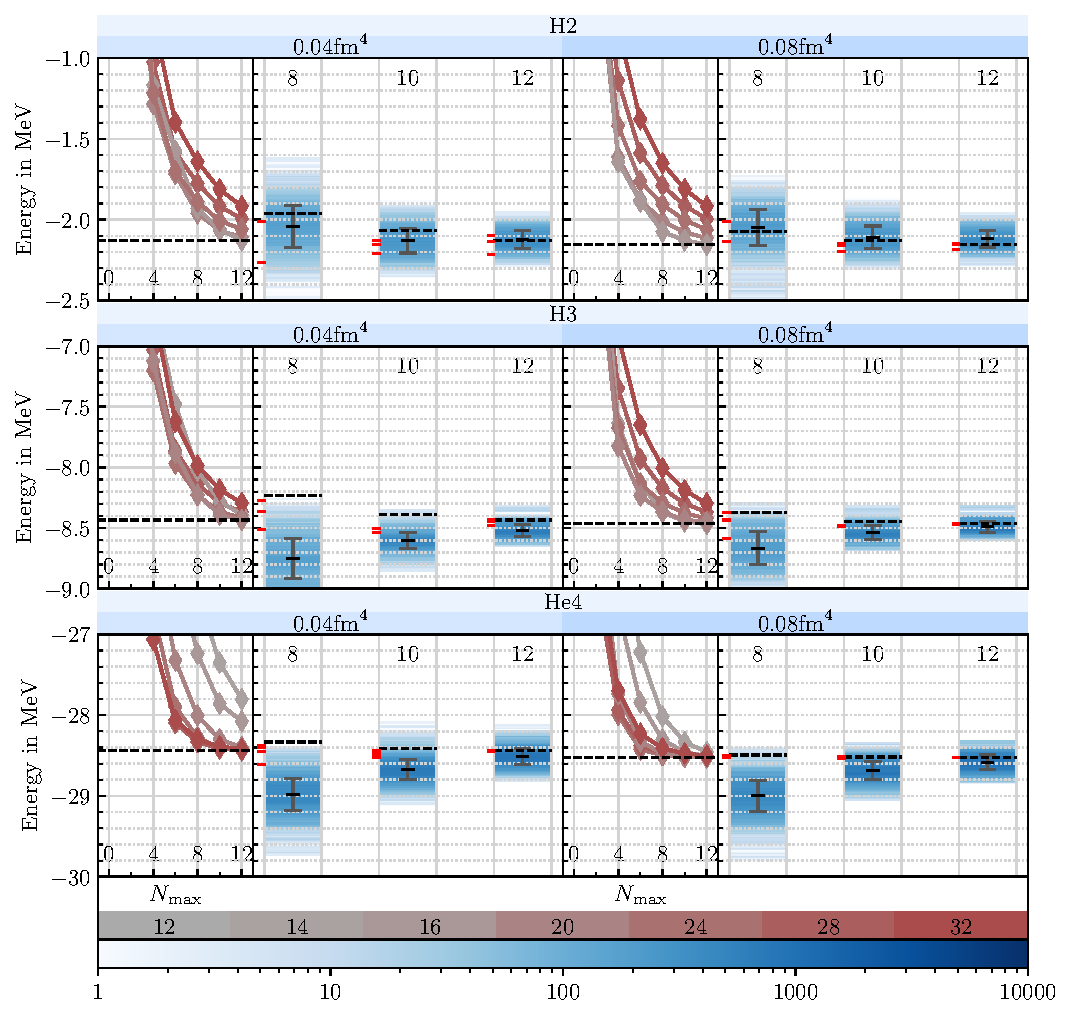
\includegraphics[width=\textwidth]{media/vanilla_evaluation_ohne_fehlfit.pdf}
  \caption{Evaluation of our extrapolation method on the nuclei \n{2}{H}, \n{3}{H} and \n{4}{He}, using a semi-local momentum space regulated N$^{2}$LO interaction with two-body interactions and a cutoff at \SI{450}{\mega\electronvolt} \cite{smsquelle}. For each nucleus and each flow parameter, the NCSM sequences are shown on the left (the different frequencies are colored respectively to the legend, which shows the frequencies $\hbar\Omega$ in \si[]{\mega\electronvolt}) and the extrapolations for a given maximum $N_\mathrm{max}$ on the right. For each maximum $N_\mathrm{max}$, the variational boundary is shown as a dashed line, and the classical extrapolations are shown as red ticks.}
  \label{fig:eval_vanilla}
\end{figure}

% Better with higher Nmax
On first sight, the network predictions get more precise when we restrict the evaluation samples to higher values of $N_\mathrm{max}$. This indicates that the networks associate steeper slopes of energy sequences with sequences that are not converged already as well as flat sequences with sequences that are more converged. Based on this, the network tries to extrapolate the steeper sequences with lower predictions and flatter sequences with higher predictions, that lie more closely to the variational boundary. In fact, for the lower values of $N_\mathrm{max}$, the networks generally predict a value for the ground-state energy which is too low in comparison to the variational boundary at the given $N_\mathrm{max}$ or even the variational boundary for the highest available $N_\mathrm{max}$, which is drawn as a dashed line on the left side of the plots.

Additionally, since the sequences for the different oscillator frequencies converge at different rates, they are further apart for lower $N_\mathrm{max}$ and thus the network extrapolates them on a broader range of energies, resulting in a bigger uncertainties for smaller $N_\mathrm{max}$.

% H2 vs rest -> slowest to converge?
An exception to this general extrapolation behavior of extrapolating unreasonably low values for smaller $N_\mathrm{max}$ and correcting the predictions towards the variational boundary for higher $N_\mathrm{max}$ is the nucleus \n{2}{H}. Here, our network shows a systematically different extrapolation behavior. First, the networks extrapolate the energies not far enough for all $N_\mathrm{max}$. Secondly, the predictions generally get lower if the maximum $N_\mathrm{max}$ of the evaluation samples is increased. This may originate from the fact that the NCSM calculations for \n{2}{H} are the slowest to converge among the three nuclei. The slow convergence results in some sequences having a much flatter slope while still being too high in value with respect to the variational boundary, which is determined by the fastest converging sequence. Another possible origin of this systematic difference is that the training set of nuclei is not balanced evenly between the nuclei and \n{2}{H} may be underrepresented, such that the slow convergence behavior of \n{2}{H} is foreign to the networks.

% 0.04 vs 0.08
If we look at the differences between the two SRG flow parameters of \srg{0.04} and \srg{0.08}, we cannot find a systematic differences but a general shift of the extrapolations to higher values with respect to their variational boundaries. This is not surprising, since a higher SRG flow parameter leads to faster convergence of the NCSM sequences. It results in lower variational boundaries as well as in a higher extrapolation, which is an effect we already observed in the \n{2}{H} extrapolations.

\section{Comparison with Classical Extrapolations}
In this section, we want to compare our extrapolation framework to a classical approach of extrapolating NCSM sequences. For that, exponential function fits as described in \autoref{sec:classical_extrapolation} are used to extrapolate the limit value of the sequences. The resulting extrapolation values are shown as red tickmarks in \autoref{fig:eval_vanilla} for each maximum $N_\mathrm{max}$.

We first look at the exponential extrapolations of \n{3}{H} and \n{4}{He}. For all $N_\mathrm{max}$, the exponential fit results in a much smaller uncertainty of the fitted limits. Furthermore, the exponential extrapolations do not violate the variational boundary condition for those $N_\mathrm{max}$. Generally, the exponential extrapolations lie way closer to the variational boundary than the extrapolations from our framework. Since the evaluated sequences converge fast (the convergence can already be seen for the higher oscillator frequencies at the higher $N_\mathrm{max}$ values), the variational bound gives a good estimate on the actual ground-state energy and thus, the exponential seem to be very accurate. This is reinforced by the fact that the exponential fits get more precise for the higher SRG flow parameter. This can especially be seen in the $N_\mathrm{max}=8$ point for \n{4}{He}. For the nuclei \n{3}{H} and \n{4}{He}, the exponential fits clearly outperform our extrapolation framework for all $N_\mathrm{max}$.

Considering the fact that the NCSM calculations, from which those extrapolations base off, already converge fast, those nuclei provide ideal conditions for the exponential extrapolations. As such, those nuclei do not represent an actual use case for extrapolations, since they are not needed for converged NCSM results. To better compare the two extrapolation methods, we look at the extrapolations of \n{2}{H}, which provides a more realistic use case, as the NCSM results do not converge as fast. Here, we see that both extrapolation methods are very comparable, both in precision and in accuracy. Interestingly, even the classical extrapolations violate the variational boundary condition for all $N_\mathrm{max}$ except $N_\mathrm{max} = 10$ for \srg{0.04}. This seems unlogical at first, since exponential fits should naturally enforce a monotonicity constraint on the extrapolated limit. Actually, the exponential fits that result in a too high prediction are coming from the sequences, for which the sequences have not converged as much. Since the variational boundary is determined by the frequencies for which the sequence has converged the most, it is possible for some sequences to result in a prediction which violates the variational boundary condition. This indicates that the violation of the network extrapolations do not come from an unoptimized training with unbalanced input sequences, but from the fact that the sequences are slow to converge. Also, NCSM calculations for the ground-state energy generally do not show an exponential convergence, which will lead to an increased uncertainty for lower $N_\mathrm{max}$. Since the exponential fits force a lower limit than the value at the highest $N_\mathrm{max}$, it is guaranteed that at least one prediction is lower than the variational boundary.

An important difference between the exponential fits and our extrapolation framework is a preconditioning of some sort for the input sequences. For the exponential function fits, this preconditioning consists of only using the best sequence, i.e. the sequence that has the lowest energy value at the highest $N_\mathrm{max}$, for the extrapolation. In our extrapolation framework, we intentionally do not preselect the "best" sequences in order to provide a more general extrapolation tool that does not depend on any sort of preselecting, which requires a metric on what sequences to pick for extrapolating the ground-state energy. In that regard, our extrapolation framework produces promisable results for unconverged sequences, as they are already comparable in quality to the classical extrapolations.

